\documentclass[border=15pt]{standalone}
\usepackage{tikz}
\usepackage{xcolor}
\usepackage{fontawesome5}

\usetikzlibrary{shapes.geometric, arrows.meta, positioning, decorations.pathreplacing, shadows, fit, shapes.symbols, calc, backgrounds}

% Nature Methods publication-quality color palette
\definecolor{natureblue}{RGB}{0, 114, 178}      % Primary blue
\definecolor{naturered}{RGB}{213, 94, 0}        % Primary red  
\definecolor{naturegreen}{RGB}{0, 158, 115}     % Primary green
\definecolor{natureyellow}{RGB}{240, 228, 66}   % Primary yellow
\definecolor{naturepurple}{RGB}{204, 121, 167}  % Primary purple
\definecolor{lightblue}{RGB}{240, 248, 255}     % Light blue background
\definecolor{lightgreen}{RGB}{240, 255, 240}    % Light green background
\definecolor{lightred}{RGB}{255, 248, 248}      % Light red background
\definecolor{lightyellow}{RGB}{255, 255, 248}   % Light yellow background
\definecolor{darkgray}{RGB}{51, 51, 51}         % Dark gray text
\definecolor{mediumgray}{RGB}{102, 102, 102}    % Medium gray
\definecolor{lightgray}{RGB}{248, 248, 248}     % Light gray

\begin{document}
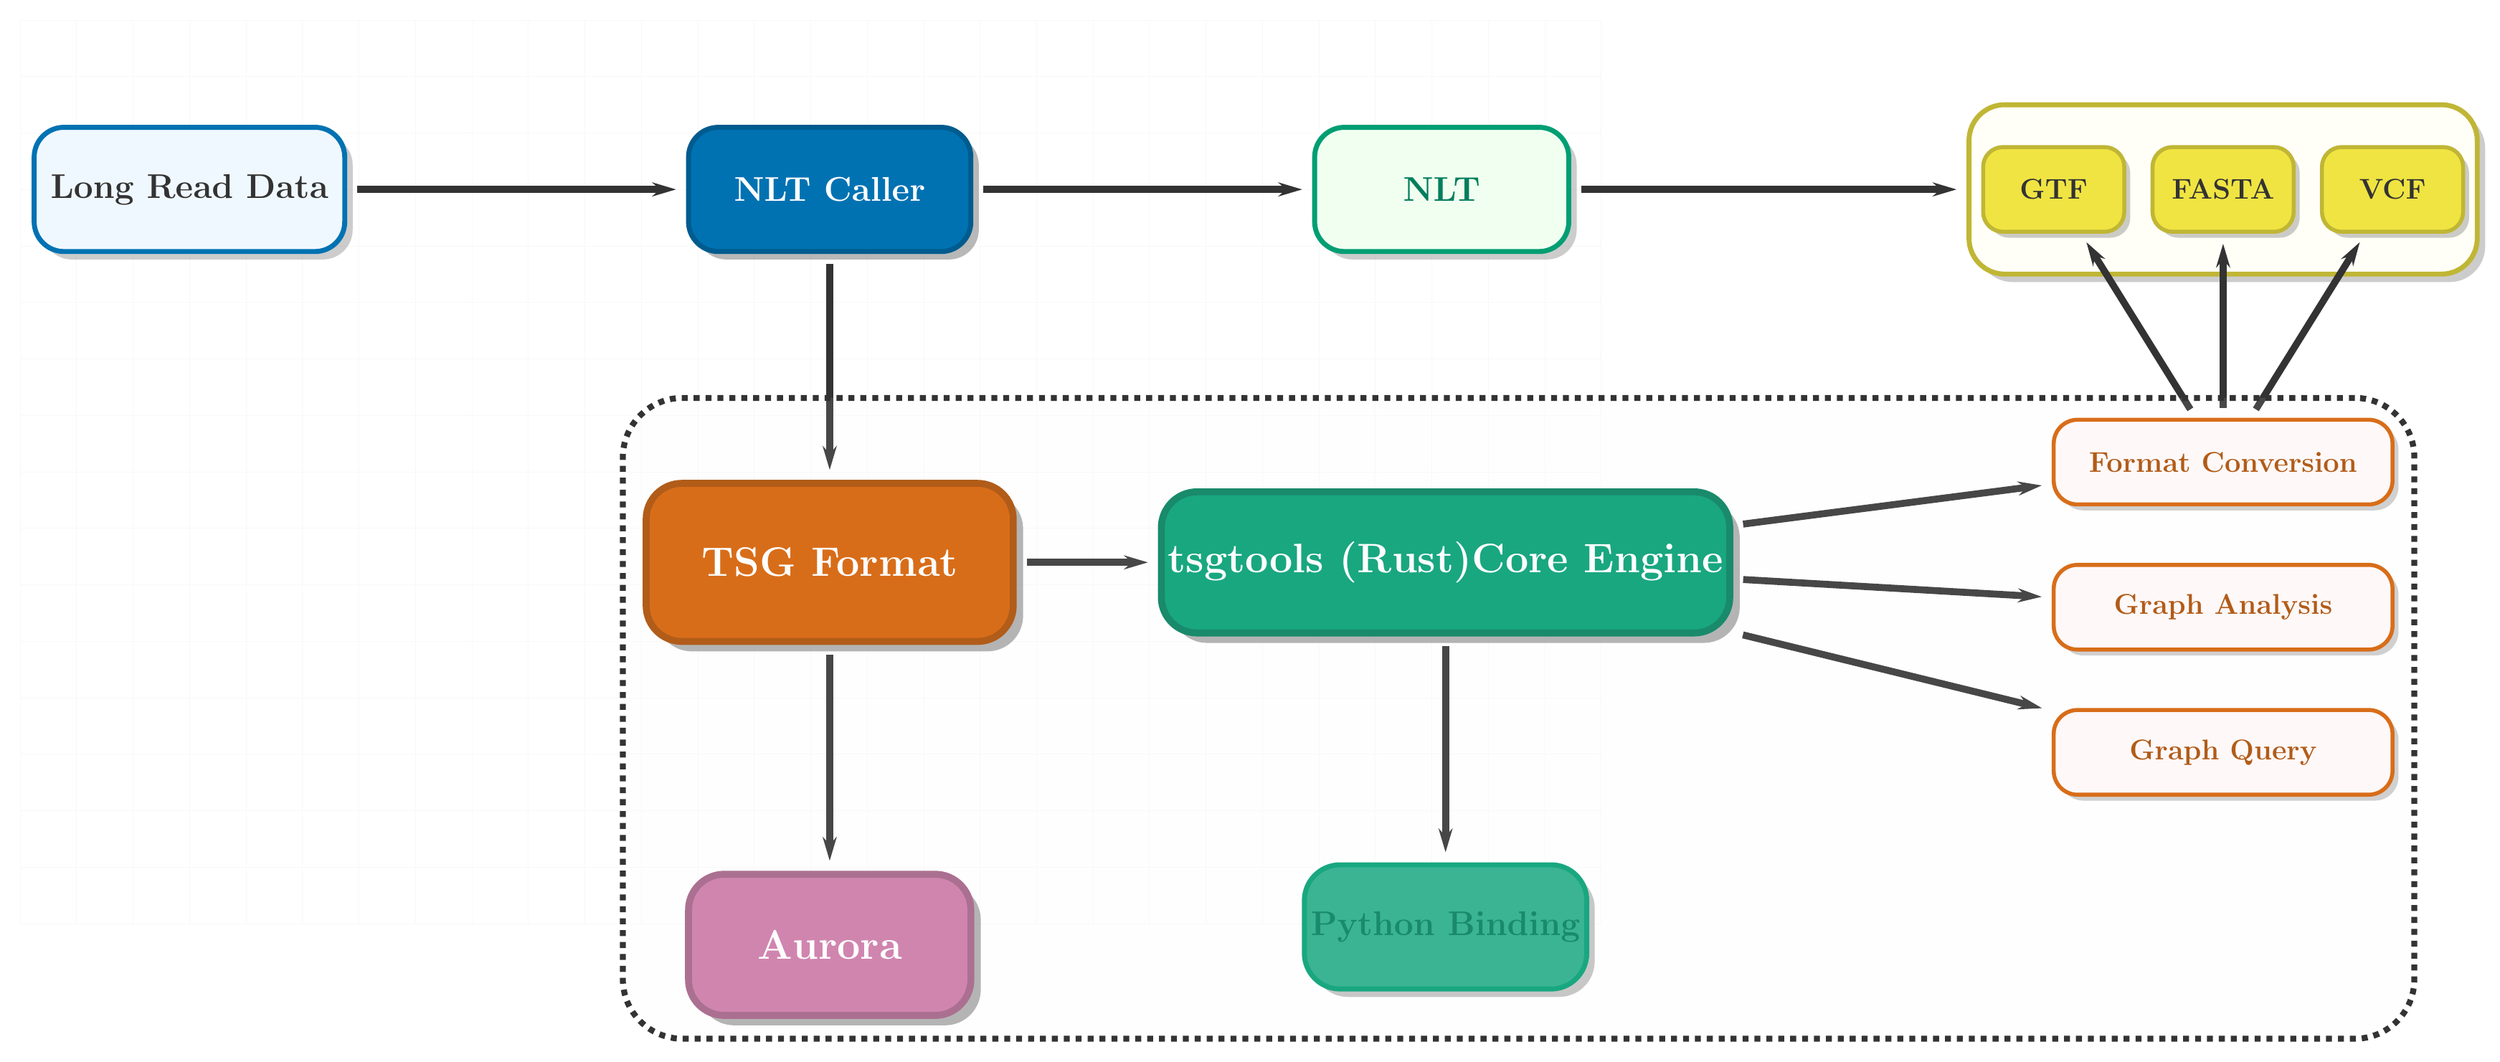
\begin{tikzpicture}[
	% Professional node styles with enhanced typography
	input/.style={
			rectangle,
			rounded corners=15pt,
			minimum width=5.5cm,
			minimum height=2.2cm,
			fill=lightblue,
			draw=natureblue,
			line width=2.5pt,
			font=\LARGE\bfseries,
			text=darkgray,
			drop shadow={shadow xshift=4pt, shadow yshift=-4pt, fill=darkgray, opacity=0.25}
		},
	caller/.style={
			rectangle,
			rounded corners=15pt,
			minimum width=5cm,
			minimum height=2.2cm,
			fill=natureblue,
			draw=natureblue!80!black,
			line width=2.5pt,
			text=white,
			font=\LARGE\bfseries,
			drop shadow={shadow xshift=4pt, shadow yshift=-4pt, fill=darkgray, opacity=0.35}
		},
	nlts/.style={
			rectangle,
			rounded corners=15pt,
			minimum width=4.5cm,
			minimum height=2.2cm,
			fill=lightgreen,
			draw=naturegreen,
			line width=2.5pt,
			text=naturegreen!80!black,
			font=\LARGE\bfseries,
			drop shadow={shadow xshift=4pt, shadow yshift=-4pt, fill=darkgray, opacity=0.25}
		},
	outputgroup/.style={
			rectangle,
			rounded corners=18pt,
			minimum width=9cm,
			minimum height=3cm,
			fill=lightyellow,
			draw=natureyellow!80!black,
			line width=2.5pt,
			drop shadow={shadow xshift=4pt, shadow yshift=-4pt, fill=darkgray, opacity=0.25}
		},
	outputbox/.style={
			rectangle,
			rounded corners=10pt,
			minimum width=2.5cm,
			minimum height=1.5cm,
			fill=natureyellow,
			draw=natureyellow!80!black,
			line width=2pt,
			font=\Large\bfseries,
			text=darkgray,
			drop shadow={shadow xshift=3pt, shadow yshift=-3pt, fill=darkgray, opacity=0.25}
		},
	tsgformat/.style={
			rectangle,
			rounded corners=18pt,
			minimum width=6.5cm,
			minimum height=2.8cm,
			fill=naturered,
			draw=naturered!80!black,
			line width=3.5pt,
			text=white,
			font=\huge\bfseries,
			drop shadow={shadow xshift=5pt, shadow yshift=-5pt, fill=darkgray, opacity=0.4}
		},
	coreengine/.style={
			rectangle,
			rounded corners=18pt,
			minimum width=7cm,
			minimum height=2.5cm,
			fill=naturegreen,
			draw=naturegreen!80!black,
			line width=3.5pt,
			text=white,
			font=\huge\bfseries,
			drop shadow={shadow xshift=5pt, shadow yshift=-5pt, fill=darkgray, opacity=0.4}
		},
	aurora/.style={
			rectangle,
			rounded corners=18pt,
			minimum width=5cm,
			minimum height=2.5cm,
			fill=naturepurple,
			draw=naturepurple!80!black,
			line width=3.5pt,
			text=white,
			font=\huge\bfseries,
			drop shadow={shadow xshift=5pt, shadow yshift=-5pt, fill=darkgray, opacity=0.4}
		},
	pythonbind/.style={
			rectangle,
			rounded corners=18pt,
			minimum width=5cm,
			minimum height=2.2cm,
			fill=naturegreen!85!white,
			draw=naturegreen,
			line width=2.5pt,
			text=naturegreen!80!black,
			font=\LARGE\bfseries,
			drop shadow={shadow xshift=4pt, shadow yshift=-4pt, fill=darkgray, opacity=0.3}
		},
	feature/.style={
			rectangle,
			rounded corners=12pt,
			minimum width=6cm,
			minimum height=1.5cm,
			fill=lightred,
			draw=naturered,
			line width=2pt,
			font=\Large\bfseries,
			text=naturered!80!black,
			drop shadow={shadow xshift=3pt, shadow yshift=-3pt, fill=darkgray, opacity=0.25}
		},
	arrow/.style={
	-{Stealth[length=12pt, width=7pt]},
	line width=3.5pt,
	color=darkgray,
	shorten >=5pt,
	shorten <=5pt
	},
	dashedarrow/.style={
	-{Stealth[length=10pt, width=6pt]},
	line width=3pt,
	color=naturegreen,
	dashed,
	shorten >=3pt,
	shorten <=3pt
	},
	ecosystembox/.style={
			rectangle,
			rounded corners=30pt,
			draw=darkgray,
			line width=3pt,
			dashed,
			fill=lightgray,
			fill opacity=0.1,
			inner sep=10pt
		},
	label/.style={
			font=\huge\bfseries,
			color=darkgray,
			text width=5cm,
			align=center,
			fill=white,
			fill opacity=0.9,
			rounded corners=8pt,
			inner sep=8pt
		}
	]

	% Top workflow row with enhanced spacing
	\node[input] (input) at (0, 10) {Long Read Data};
	\node[caller, right=6cm of input] (caller) {NLT Caller};
	\node[nlts, right=6cm of caller] (nlts) {NLT};

	% Output formats group with better organization
	\node[outputgroup, right=7cm of nlts] (outputgroup) {};
	\node[outputbox] (gtf) at ([xshift=-3cm] outputgroup.center) {GTF};
	\node[outputbox] (fasta) at (outputgroup.center) {FASTA};
	\node[outputbox] (vcf) at ([xshift=3cm] outputgroup.center) {VCF};

	% TSG Ecosystem core components with improved positioning
	\node[tsgformat, below=4cm of caller] (tsg) {TSG Format};
	\node[coreengine, right=2.5cm of tsg] (tsgtools) {tsgtools (Rust) \\Core Engine};
	\node[aurora, below=4cm of tsg] (aurora) {Aurora};
	\node[pythonbind, below=4cm of tsgtools] (python) {Python Binding};

	% Feature boxes with enhanced positioning
	\node[feature, below=2.5cm of outputgroup] (conv) {Format Conversion};
	\node[feature, below=1cm of conv] (analysis) {Graph Analysis};
	\node[feature, below=1cm of analysis] (query) {Graph Query};

	% Main workflow arrows with enhanced styling
	\draw[arrow] (input) -- (caller);
	\draw[arrow] (caller) -- (nlts);
	\draw[arrow] (nlts) -- (outputgroup);

	% Ecosystem connections with improved flow
	\draw[arrow] (caller) -- (tsg);
	\draw[arrow] (tsg) -- (tsgtools);
	\draw[arrow] (tsg) -- (aurora);
	\draw[arrow] (tsgtools) -- (python);
	\draw[arrow] (tsgtools) -- (conv);
	\draw[arrow] (tsgtools) -- (analysis);
	\draw[arrow] (tsgtools) -- (query);

	% Output connections
	\draw[arrow] (conv) -- (gtf);
	\draw[arrow] (conv) -- (fasta);
	\draw[arrow] (conv) -- (vcf);

	% % Ecosystem boundary box with enhanced styling - includes all TSG ecosystem components
	\node[ecosystembox, fit={(tsg) (python) (tsgtools) (aurora) (conv) (analysis) (query)}] (ecosystem) {};

	% Add subtle professional background
	\begin{scope}[on background layer]
		\draw[lightgray, very thin] (-3, -3) grid (25, 13);
	\end{scope}

\end{tikzpicture}
\end{document}
